\chapter{ТЕХНОЛОГИЧЕСКАЯ ЧАСТЬ}

В этом разделе будут выбраны средства реализации программного обеспечения. Будет выбран язык программирования, системы управления базами данных и программное обеспечение для графического интерфейса. Будут реализован код базы данных и будет реализовано взаимодействие между приложением и базой данных. Будет приведена демонстрация работы программы, реализующей функции каждой роли.

\section{Выбор системы управления базой данных}

Система управления базами данных --- это совокупность программных и лингвистических средств общего или специального назначения, обеспечивающих управление созданием и использованием баз данных~\cite{database}.

Предполагается, что реализуемая база данных будет хранить большое количество информации.

Система управления базой данных должна удовлетворять следующим требованиям.

\begin{enumerate}
	\item Система управления базой данных должна предоставлять такие типы данных как строки, целые числа, даты и xml, чтобы можно было хранить информацию. 
	\item Для загрузки xml файла из приложения в системе управления базой данных должна быть реализована возможность создания хранимых процедур. 
	\item Система управления базой данных должна обеспечивать надежное хранение данных, то есть данные не должны потеряться даже, если в системе произойдет сбой.
\end{enumerate} 

В качестве системы управления базой данных был выбран SQL Server, так как он удовлетворяет всем выделенным требованиям.

\section{Выбор языка программирования}

В качестве языка программирования был выбран C\#~\cite{sharp}, так как он является полностью объектно-ориентированным, что позволяет использовать наследование, интерфейсы и абстракцию. Также стандартная библиотека C\# включает пространство имен System.Data.Linq.Mapping~\cite{datalinqmapping}, которое содержит классы для формирования объектной модели LINQ to SQL, представляющей структуру и содержимое реляционной базы данных.

Для упаковки приложения как полноценного продукта была выбрана система контейнеризации Docker~\cite{docker}. Docker используется для создания изолированной среды для программного обеспечения, которое может быть развернуто на различных устройствах без дополнительной настройки.

\section{Реализация ролевой модели}

Необходимо реализовать ролевую модель в соответствии с пунктом~\ref{functions}. Роль --- это разрешение, предоставляемое группе пользователей для доступа к данным. 

Ролевая модель реализована как на уровне приложения, так и на уровне базы данных~\ref{lst:role1}. В листинге~\ref{lst:role1} приведено создание ролей для авторизованного и неавторизованного пользователей.

\captionsetup{justification=raggedright,singlelinecheck=off}
\begin{lstlisting}[label=lst:role1, caption=Ролевая модель на уровне базы данных, language=SQL]
create login [AuthorizedUser] with password = 'UserPassword1'
create user AU for login [AuthorizedUser]
create role [AuthorizedUserRole]
alter role [AuthorizedUserRole] add member AU
deny delete on Reviews to [AuthorizedUserRole];
deny update on Reviews to [AuthorizedUserRole];
deny delete on TimeRecords to [AuthorizedUserRole];
deny update on TimeRecords to [AuthorizedUserRole];
deny insert on Games to [AuthorizedUserRole];
deny delete on Games to [AuthorizedUserRole];
deny update on Games to [AuthorizedUserRole];
deny delete on Users to [AuthorizedUserRole];
deny update on Users to [AuthorizedUserRole];
deny alter to [AuthorizedUserRole];
grant insert on Reviews to [AuthorizedUserRole];
grant insert on TimeRecords to [AuthorizedUserRole];
grant insert on Users to [AuthorizedUserRole];
grant select on Users to [AuthorizedUserRole];
grant select on Games to [AuthorizedUserRole];
grant select on Reviews to [AuthorizedUserRole];
grant select on TimeRecords to [AuthorizedUserRole];

create login [GuestUser] with password = 'GuestPassword1'
create user GU for login [GuestUser]
create role [GuestUserRole]
alter role [GuestUserRole] add member GU
deny delete on Reviews to [GuestUserRole];
deny update on Reviews to [GuestUserRole];
deny delete on TimeRecords to [GuestUserRole];
deny update on TimeRecords to [GuestUserRole];
deny insert on Games to [GuestUserRole];
deny delete on Games to [GuestUserRole];
deny update on Games to [GuestUserRole];
deny delete on Users to [GuestUserRole];
deny update on Users to [GuestUserRole];
deny alter to [GuestUserRole];
deny insert on Reviews to [GuestUserRole];
deny insert on TimeRecords to [GuestUserRole];
grant insert on Users to [GuestUserRole];
grant select on Users to [GuestUserRole];
grant select on Games to [GuestUserRole];
grant select on Reviews to [GuestUserRole];
grant select on TimeRecords to [GuestUserRole];
\end{lstlisting}

\section{Реализация процедуры преобразования строки в xml формат и вставки в таблицу}

В листинге~\ref{lst:func} представлена реализация процедуры преобразования строки с перечислением жанров в xml формат и вставки в таблицу Games на уровне базы данных. 

\begin{lstlisting}[label=lst:func, caption=Процедура преобразования строки в xml формат и вставки в таблицу на уровне базы данных,language=SQL]
create or alter procedure InsertGameProcedure
(
	@title nvarchar(200),
	@releaseDate date,
	@developer nvarchar(200),
	@publisher nvarchar(200),
	@genres nvarchar(200)
)
as
begin
	delete temp where 0 = 0
	insert into temp
	select @title, genre_split.value
	from string_split(@genres, ' ') as genre_split

	insert into Games
	values(@title, @releaseDate, @developer, @publisher,
	(
		select temp.genre
		from temp
		for xml path(''), type, root('Genre')
	))
	delete temp where 0 = 0
end
\end{lstlisting}

В листинге~\ref{lst:strtoxml} приведена реализация процедуры преобразования строки с перечислением жанров в xml формат и вставки в таблицу Games на уровне приложения.

\begin{lstlisting}[label=lst:strtoxml, caption=Метод преобразования строки в xml формат и вставки в таблицу на уровне приложения]
public void AddGameXMLApp(Game game)
{
	DataContext db = new DataContext(adminConnection);
	Table<GamesXML> gameTable = db.GetTable<GamesXML>();
	XmlDocument xml = GetXml(game.Genres);
	GamesXML g = new GamesXML()
	{
		Title = game.Title,
		ReleaseDate = game.ReleaseDate,
		Developer = game.Developer,
		Publisher = game.Publisher,
		Genres = xml.InnerXml,
	};
	gameTable.InsertOnSubmit(g);
	try
	{
		db.SubmitChanges();
	}
	catch (DuplicateKeyException e)
	{
		throw new GameAlreadyExistsException(e.Message);
	}
}

XmlDocument GetXml(string genres)
{
	string[] genreSplit = genres.Split(' ');
	XmlDocument xml = new XmlDocument();
	XmlElement root = xml.CreateElement("Genres");
	xml.AppendChild(root);
	foreach (var genre in genreSplit)
		xml["Genres"].AppendChild(xml.CreateElement("genre")) .InnerText = genre;
	return xml;
}
\end{lstlisting}

\section{Реализация модели <<Отзыв>>}

В листинге~\ref{lst:reviews} приведено создание таблицы Reviews в базе данных, а также создание ограничений целостности. 

\begin{lstlisting}[label=lst:reviews, caption=Таблица Reviews, language=SQL]
create table Reviews
(
	GameId int,
	UserLogin nvarchar(200),
	[Text] nvarchar(1000),
	Score int,
	PublicationDate date,
	primary key(GameId, UserLogin)
);
\end{lstlisting}

В листинге~\ref{lst:review} представлена реализация модели Review, которая реализует соответствующую сущность в компоненте бизнес-логики.

\begin{lstlisting}[label=lst:review, caption=Модель Review]
public class Review
{
	public int GameId { get; }
	public string UserLogin { get; }
	public uint Score { get; }
	public string Text { get; }
	public DateTime PublicationDate { get; }
	public Review(int gameId, string userLogin, uint score, string text, DateTime publicationDate)
	{
		GameId = gameId;
		UserLogin = userLogin;
		Score = score;
		Text = text;
		PublicationDate = publicationDate;
	}
}
\end{lstlisting}

В листинге~\ref{lst:reviewRep} приведена реализация репозитория, который предоставляет доступ к данным таблицы Reviews из базы данных. 

\captionsetup{justification=raggedleft,singlelinecheck=off}
\begin{lstlisting}[label=lst:reviewRep, caption=Репозиторий SqlServerReviewRepository доступа к таблице Reviews из базы данных]
[Table]
public class Reviews
{
	[Column(IsPrimaryKey = true)]
	public int GameId { get; set; }
	[Column(IsPrimaryKey = true)]
	public string UserLogin { get; set; }
	[Column]
	public string Text { get; set; }
	[Column]
	public int Score { get; set; }
	[Column]
	public DateTime PublicationDate { get; set; }
}

public class SqlServerReviewRepository : SqlServerRepository, IReviewRepository
{
	public SqlServerReviewRepository() : base() { }
	
	public void AddReview(Review review)
	{
		DataContext db = new DataContext(userConnection);
		Table<Reviews> reviewTable = db.GetTable<Reviews>();
		Reviews r = new Reviews()
		{
			GameId = review.GameId,
			UserLogin = review.UserLogin,
			Score = (int)review.Score,
			Text = review.Text,
			PublicationDate = review.PublicationDate
		};
		reviewTable.InsertOnSubmit(r);
		db.SubmitChanges();
	}
	
	public void DeleteReview(Review review)
	{
		DataContext db = new DataContext(adminConnection);
		Reviews rev = db.GetTable<Reviews>().Where(r => r.GameId == review.GameId && r.UserLogin == review.UserLogin).First();
		db.GetTable<Reviews>().DeleteOnSubmit(rev);
		db.SubmitChanges();
	}
	
	public List<Review> GetReviews(int id)
	{
		DataContext db = new DataContext(guestConnection);
		IQueryable<Reviews> gameReviews = from r in db.GetTable<Reviews>()
		where r.GameId == id
		select r;
		List<Review> reviews = new List<Review>();
		foreach (var rev in gameReviews)
		reviews.Add(new Review(rev.GameId, rev.UserLogin, (uint)rev.Score, rev.Text, rev.PublicationDate));
		return reviews;
	}
}
\end{lstlisting}

\section{Демонстрация интерфейса приложения}

На рисунке~\ref{img:main} показан интерфейс приложения при запуске, библиотека видеоигр. Пользователь не авторизован. Пользователь может только авторизоваться, зарегистрироваться и посмотреть информацию и статистику об игре.

\clearpage
\begin{figure}[H]
	\begin{center}
		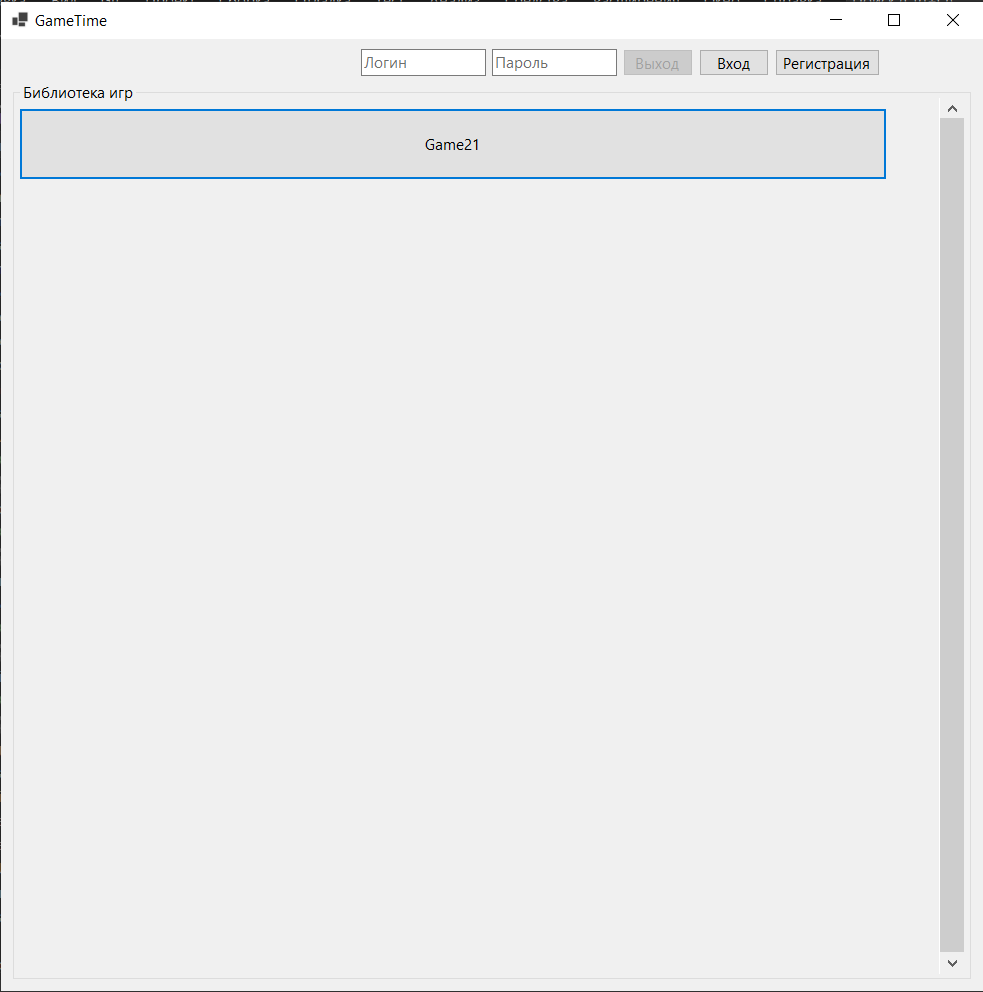
\includegraphics[scale=0.7]{../imgs/interface/main.png}
	\end{center}
	\captionsetup{justification=centering}
	\caption{Библиотека видеоигр}
	\label{img:main}
\end{figure}

На рисунках~\ref{img:gamePageGuest},~\ref{img:gamePageUser},~\ref{img:gamePageAdmin} показана страница игры, которая доступна неавторизованному, авторизованному пользователю и администратору соответственно.

\begin{figure}[H]
	\begin{center}
		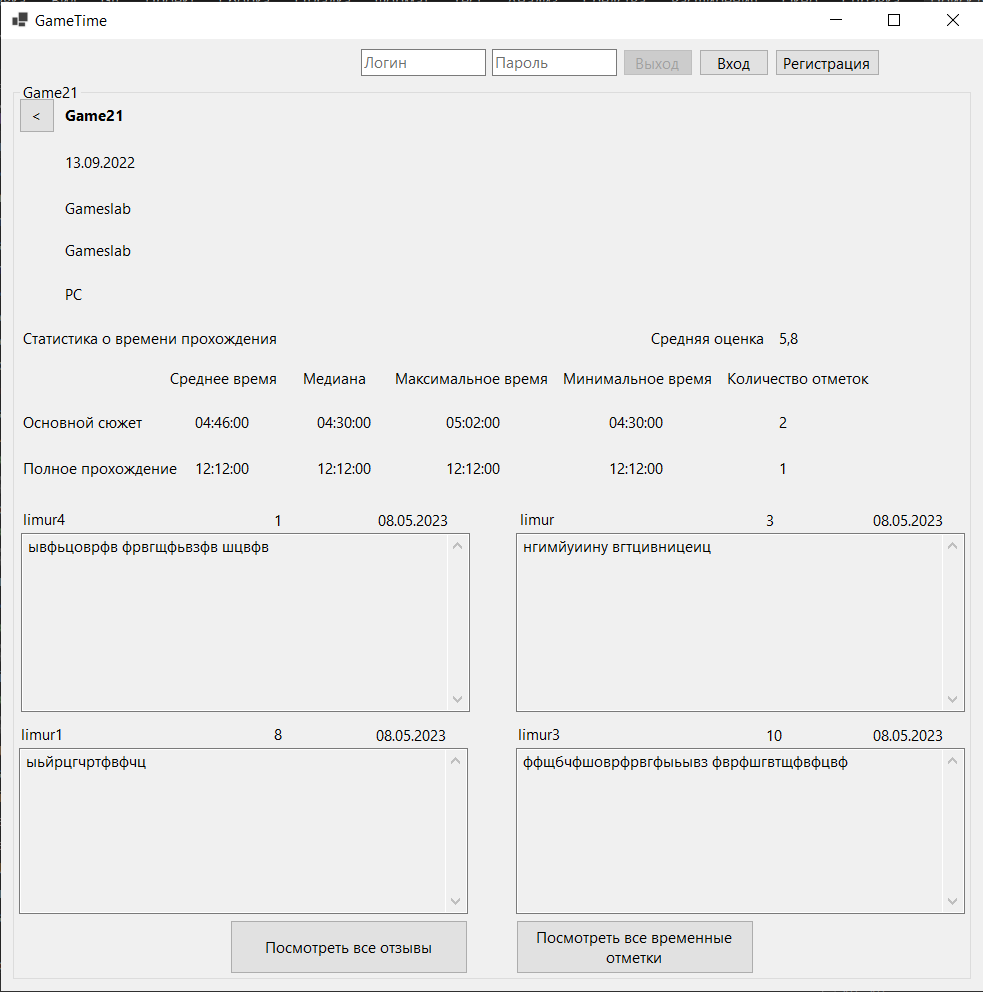
\includegraphics[scale=0.7]{../imgs/interface/gamePageGuest.png}
	\end{center}
	\captionsetup{justification=centering}
	\caption{Страница игры, которую видит не авторизованный пользователь}
	\label{img:gamePageGuest}
\end{figure}

\begin{figure}[H]
	\begin{center}
		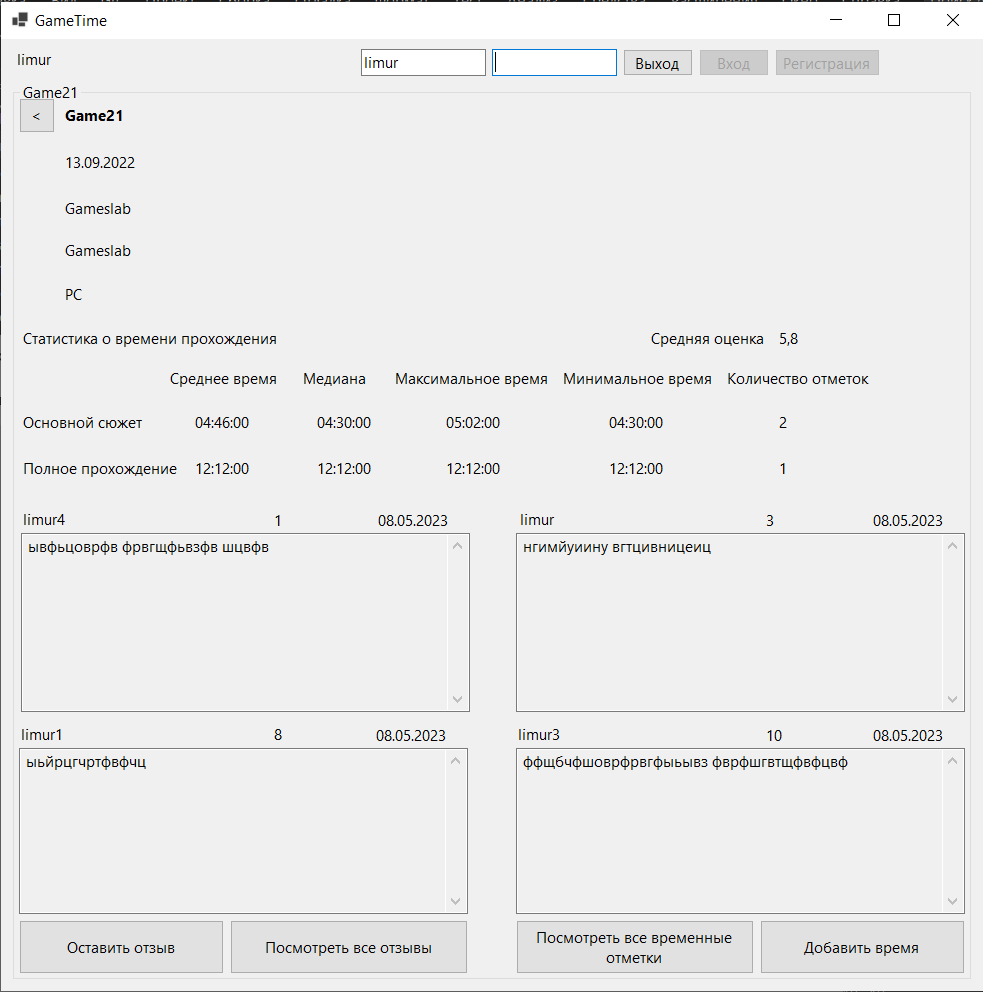
\includegraphics[scale=0.7]{../imgs/interface/gamePageUser.png}
	\end{center}
	\captionsetup{justification=centering}
	\caption{Страница игры, которую видит авторизованный пользователь}
	\label{img:gamePageUser}
\end{figure}

\begin{figure}[H]
	\begin{center}
		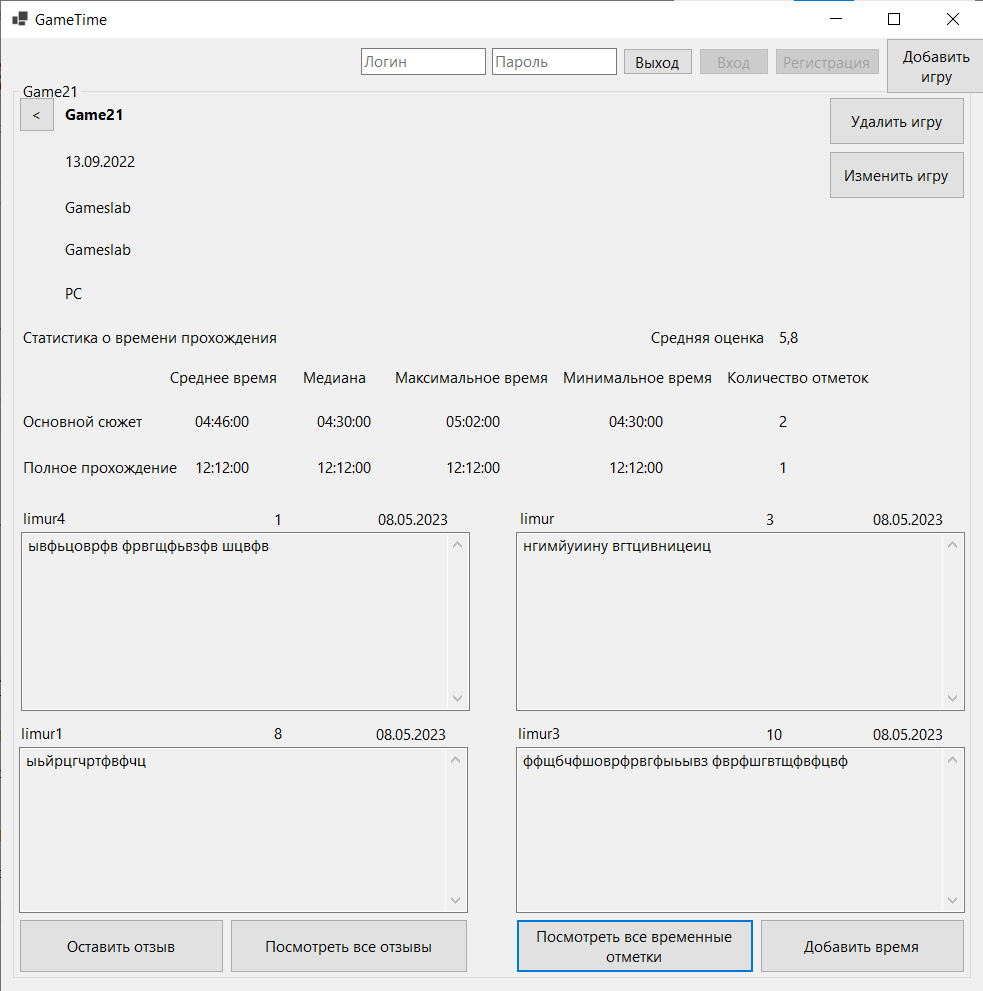
\includegraphics[scale=0.7]{../imgs/interface/gamePageAdmin.png}
	\end{center}
	\captionsetup{justification=centering}
	\caption{Страница игры, которую видит администратор}
	\label{img:gamePageAdmin}
\end{figure}

На рисунке~\ref{img:addTimeRecord} показан интерфейс окна, в котором можно добавить временную отметку игре. 


\begin{figure}[H]
	\begin{center}
		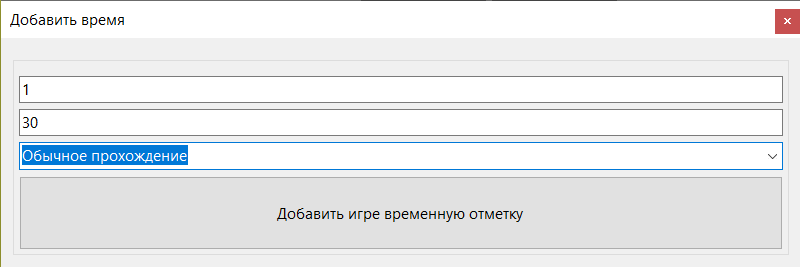
\includegraphics[scale=0.8]{../imgs/interface/addTimeRecord.png}
	\end{center}
	\captionsetup{justification=centering}
	\caption{Окно для добавления временной отметки игре}
	\label{img:addTimeRecord}
\end{figure}
\clearpage

На рисунке~\ref{img:addReview} показан интерфейс окна, в котором можно добавить отзыв об игре. 

\begin{figure}[H]
	\begin{center}
		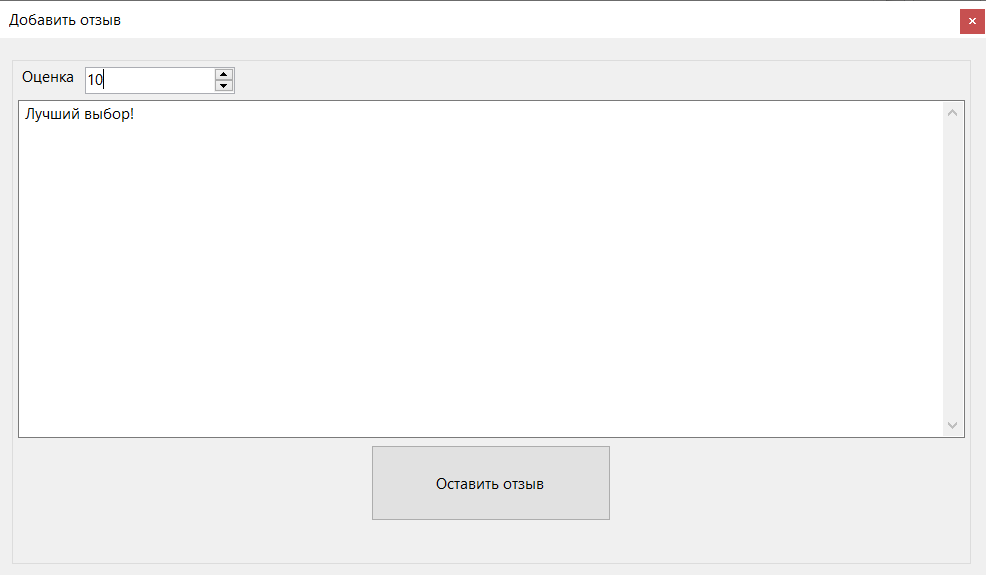
\includegraphics[scale=0.7]{../imgs/interface/addReview.png}
	\end{center}
	\captionsetup{justification=centering}
	\caption{Окно для добавления отзыва об игре}
	\label{img:addReview}
\end{figure}

На рисунке \ref{img:allTimeRecordU} показан интерфейс окна, в котором можно посмотреть все временные отметки игры. Администратору доступно удаление конкретной, что показано на рисунке~\ref{img:allTimeRecordA}.

\clearpage
\begin{figure}[H]
	\begin{center}
		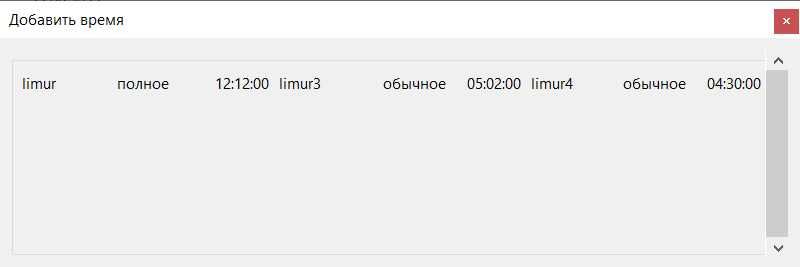
\includegraphics[scale=0.8]{../imgs/interface/AllTimeRecordsU.png}
	\end{center}
	\captionsetup{justification=centering}
	\caption{Все временные отметки игры}
	\label{img:allTimeRecordU}
\end{figure}

\begin{figure}[H]
	\begin{center}
		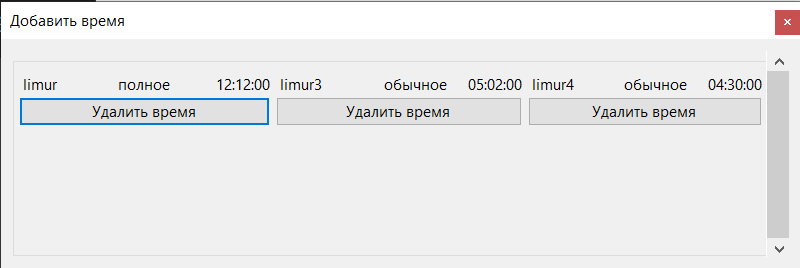
\includegraphics[scale=0.8]{../imgs/interface/AllTimeRecordsA.png}
	\end{center}
	\captionsetup{justification=centering}
	\caption{Все временные отметки игры (администратор)}
	\label{img:allTimeRecordA}
\end{figure}

На рисунке \ref{img:allReviewsU} показан интерфейс окна, в котором можно посмотреть все отзывы игры. Администратору доступно удаление конкретного, что показано на рисунке~\ref{img:allReviewsA}.

\begin{figure}[H]
	\begin{center}
		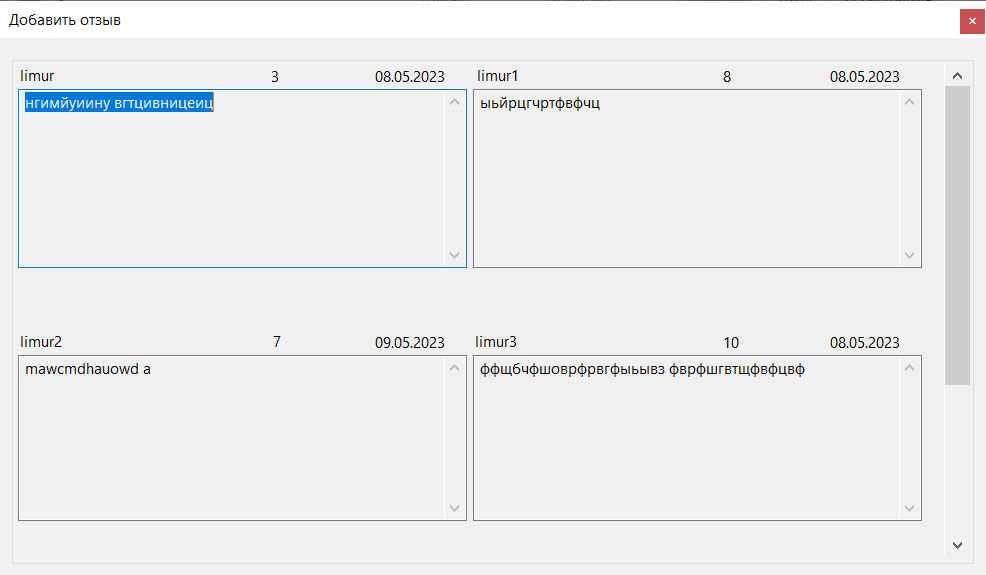
\includegraphics[scale=0.7]{../imgs/interface/AllReviewsU.png}
	\end{center}
	\captionsetup{justification=centering}
	\caption{Все отзывы игры}
	\label{img:allReviewsU}
\end{figure}

\begin{figure}[H]
	\begin{center}
		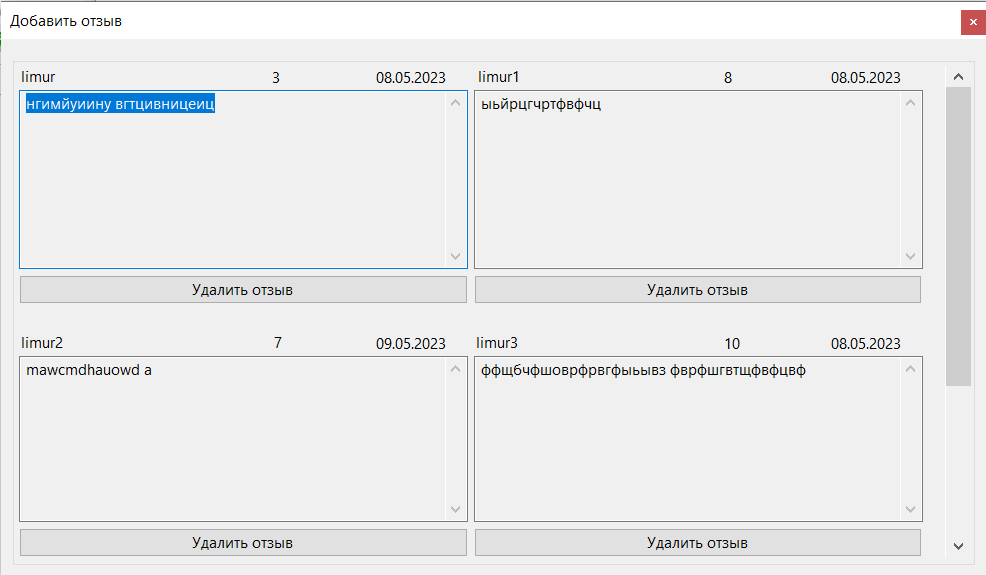
\includegraphics[scale=0.7]{../imgs/interface/AllReviewsA.png}
	\end{center}
	\captionsetup{justification=centering}
	\caption{Все отзывы игры (администратор)}
	\label{img:allReviewsA}
\end{figure}

На рисунке~\ref{img:addGame} представлен интерфейс окна для добавления или изменения игры.

\begin{figure}[H]
	\begin{center}
		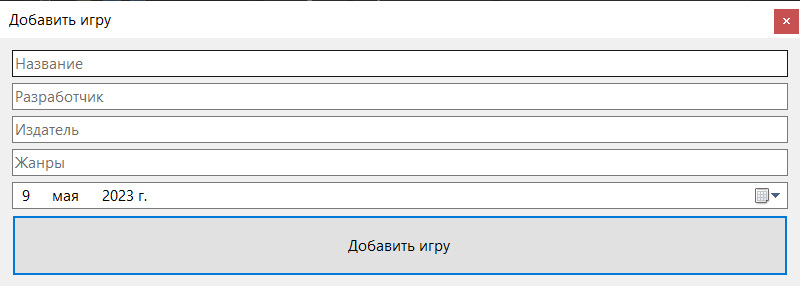
\includegraphics[scale=0.8]{../imgs/interface/AddGame.png}
	\end{center}
	\captionsetup{justification=centering}
	\caption{Окно добавления игры}
	\label{img:addGame}
\end{figure}

\section{Тестирование приложения}

Тестирование проводилось по методологии черного ящика. Для тестирования компонента бизнес-логики была использована такая технология тестирования, как unit-тесты. Для тестирования взаимодействие компонента доступа к данным и базы данных были написаны интеграционные тесты. Система тестирования была реализована с помощью фреймворка MS Test~\cite{mstest}, которая позволяет быстро и автоматически протестировать отдельные компоненты приложения независимо от остальной его части. 